\documentclass[]{report}
\usepackage{listings}
\usepackage{booktabs}
\usepackage{float}
\usepackage{graphicx}
\usepackage{color}   %May be necessary if you want to color links
\usepackage{hyperref}
\usepackage{amsmath}
\usepackage{nccmath}
\hypersetup{
    colorlinks=true,
    linktoc=all,     
    linkcolor=blue,  
}
\lstset{basicstyle=\fontsize{10}{10}\selectfont\ttfamily}

\title{Modeling Sorting Algorithms in Different Programming Languages} 
\author{Hamza Rehioui} 
\date{\today}

\begin{document} 
    \maketitle
	\begin{abstract}
		As a part of my final project for the Introduction to Mathematical Modeling class with Dr. Van Nguyen, I decided to study how two sorting algorithms - bubble sort and merge sort - behave across three different programming languages. My choice of programming languages was based on having different paradigms: C as the imperative paradigm, Python as the object oriented paradigm, and finally, Racket for the functional paradigm. This would in turn give me an idea on how time complexities behave and how actual durations fare in front of expected ones.
	\end{abstract}
	
	\tableofcontents
	\listoffigures
	\listoftables
	
	\pagebreak
    
    \chapter{Introduction}
    
    	\section{Programming Languages}
	    In this research project, I will be using multiple programming languages to conduct my study. More specifically, I will be using C, Python, and Racket for the comparison, and R is the statistical tool used as a means of comparison and analysis.
	    	\subsection{C Language}
	    	C is a high-level and general-purpose programming language that is ideal for developing firmware or portable applications. Originally intended for writing system software, C was developed at Bell Labs by Dennis Ritchie for the Unix Operating System in the early 1970s. \cite{techopedia_2018}
	    	\subsection{Python}
	    	Python is a computer programming language often used to build websites and software, automate tasks, and conduct data analysis. Python is a general-purpose object-oriented language, meaning it can be used to create a variety of different programs and isn’t specialized for any specific problems. This versatility, along with its beginner-friendliness, has made it one of the most-used programming languages today. \cite{coursera}
	    	\subsection{Racket}
	    	Racket falls into a broad category of programming languages often called functional programming languages. Functional refers to a focus on functions in the mathematical sense. Unfortunately, the term can be a bit confusing, since many other languages (such as the widely-known C language) use constructs called functions, even though they do not follow a “functional” style. Functional languages are built around the evaluation of expressions and the application of functions for their results, rather than the execution of sequences of commands for their effects on stored data. In some sense, functional languages are a little closer to expressing what to compute, while imperative (command-, statement-, and assignment-focused) languages are closer to expressing how to compute it. Functional languages are closer to math; imperative languages are closer to the model presented by most modern computer hardware systems. \cite{cs 251: racket}
	    	\subsection{R Language}
	    	R is a programming language for statistical computing and graphics supported by the R Core Team and the R Foundation for Statistical Computing. Created by statisticians Ross Ihaka and Robert Gentleman, R is used among data miners and statisticians for data analysis and developing statistical software. Users have created packages to augment the functions of the R language. \cite{wikipedia_2022:2}
	    	
	    \section{Algorithms}
	    In this study, I have chosen two algorithms with different time complexities and varying difficulty: Bubble Sort and Merge Sort.
	    	\subsection{Bubble Sort}
	    	Bubble sort is a sorting algorithm that compares two adjacent elements and swaps them until they are not in the intended order. Just like the movement of air bubbles in the water that rise up to the surface, each element of the array move to the end in each iteration. Therefore, it is called a bubble sort. \cite{programiz}
	    	\subsection{Merge Sort}
	    	Merge Sort is a Divide and Conquer algorithm. It divides the input array into two halves, calls itself for the two halves, and then merges the two sorted halves. The merge() function is used for merging two halves. The merge(arr, l, m, r) is a key process that assumes that arr[l..m] and arr[m+1..r] are sorted and merges the two sorted sub-arrays into one. See the following C implementation for details. \cite{geeksforgeeks_2022}


	 \chapter{Data Collection}
	 	In order to conduct my data collection phase, I had to write out a merge sort and a bubble sort in all three languages.
	 	\section{Algorithm Codes}
			\subsection{C Language}
		 		\subsubsection{Bubble Sort}
		 		
		 		\lstinputlisting[language=C]{resources/algorithms/codeinc.c}
		 		
		 		\subsubsection{Merge Sort}
		 		
		 		\lstinputlisting[language=C]{resources/algorithms/mcodeinc.c}
		 		
		 	\subsection{Python}
		 		\subsubsection{Bubble Sort}
		 		
		 		\lstinputlisting[language=Python]{resources/algorithms/codeinpy.py}
		 		
		 		\subsubsection{Merge Sort}
		 		
		 		\lstinputlisting[language=Python]{resources/algorithms/mcodeinpy.py}
		 		
		    \subsection{Racket}
		 		\subsubsection{Bubble Sort}
		 		
		 		\lstinputlisting[language=Lisp]{resources/algorithms/codeinrkt.rkt}
		 		
		 		\subsubsection{Merge Sort}
		 		
		 		\lstinputlisting[language=Lisp]{resources/algorithms/mcodeinrkt.rkt}
			
		\section{Testing Codes}
		While now we know how the algorithms are laid out in all three languages, we still need the testing code that would generate arrays of custom length of random numbers and benchmark the time taken to run one sorting instance on that array. In this section, I will run display all testing codes.
			\subsection{C Language}
		 		\subsubsection{Bubble Sort}
		 		
		 		\lstinputlisting[language=C]{resources/testing/codeinctesting.c}
		 		
		 		\subsubsection{Merge Sort}
		 		
		 		\lstinputlisting[language=C]{resources/testing/mcodeinctesting.c}
		 		
		 	\subsection{Python}
		 		\subsubsection{Bubble Sort}
		 		
		 		\lstinputlisting[language=Python]{resources/testing/codeinpytesting.py}
		 		
		 		\subsubsection{Merge Sort}
		 		
		 		\lstinputlisting[language=Python]{resources/testing/mcodeinpytesting.py}
		 		
		    \subsection{Racket}
		 		\subsubsection{Bubble Sort}
		 		
		 		\lstinputlisting[language=Lisp]{resources/testing/codeinrkttesting.rkt}
		 		
		 		\subsubsection{Merge Sort}
		 		
		 		\lstinputlisting[language=Lisp]{resources/testing/mcodeinrkttesting.rkt}
		 		
		    \subsection{Bash Script}
		    Finally, to run all of these tests, I have set up a BASH script to run on my computer and run four trials for each and every code.
		    	
		    	\lstinputlisting[language=bash]{resources/testing/bash.sh}
	  
	  
		\section{Test Results}
		Once I finished testing both the algorithms and the testing code, I had to move on the actual data collection. In this section, I will run 4 trials on all three languages and average them out to find an average running time for each algorithm in each language. Later on in my paper, I will graph this dataset using R tools.
			\subsection{C Language}
		 		\subsubsection{Bubble Sort}
		 		
		 		\begin{table}[H]  
  				  \centering
  				  \caption{Bubble Sort in C}
		 		  \begin{tabular}{cccccc}
		 		    \toprule
		 		         & \textbf{Trial 1} & \textbf{Trial 2} & \textbf{Trial 3} & \textbf{Trial 4} & \textbf{Average} \\ \midrule
		 		    \textbf{100}   & 0.000030 & 0.000030 & 0.000028 & 0.000033 & 0.000030   \\
		 		    \textbf{1000}  & 0.002364 & 0.002238 & 0.002207 & 0.003026 & 0.002459   \\
		 		    \textbf{10000} & 0.314041 & 0.314055 & 0.315845 & 0.386813 & 0.332689   \\
		 		    \textbf{12500} & 0.501716 & 0.491243 & 0.493394 & 0.621091 & 0.526861   \\
		 		    \textbf{15000} & 0.741801 & 0.714311 & 0.716607 & 0.925301 & 0.774505   \\
		 		    \textbf{20000} & 1.293619 & 1.281955 & 1.291895 & 1.638969 & 1.376610   \\
		 		    \textbf{30000} & 2.946970 & 2.941916 & 2.963792 & 3.636154 & 3.122208   \\
		 		    \textbf{40000} & 5.290429 & 5.275138 & 5.821433 & 5.374234 & 5.440309   \\
		 		    \textbf{50000} & 8.305266 & 8.303268 & 8.482247 & 8.306714 & 8.349374   \\
		 		    \textbf{60000} & 11.950539 & 12.098505 & 13.396408 & 12.014277 & 12.364932   \\ \bottomrule
		 		  \end{tabular}
		 		\end{table}

		 		\subsubsection{Merge Sort} 
		 		
				\begin{table}[H]  
  				  \centering
  				  \caption{Merge Sort in C}
		 		  \begin{tabular}{cccccc}
		 		    \toprule
		 		         & \textbf{Trial 1} & \textbf{Trial 2} & \textbf{Trial 3} & \textbf{Trial 4} & \textbf{Average} \\ \midrule
		 		    \textbf{100} 	& 0.000013 & 0.000014 & 0.000013 & 0.000013 & 0.000013   \\
		 		    \textbf{1000} 	& 0.000137 & 0.000136 & 0.000141 & 0.000200 & 0.000154   \\
		 		    \textbf{10000} 	& 0.001786 & 0.001721 & 0.001792 & 0.001778 & 0.001769   \\
		 		    \textbf{100000} & 0.021886 & 0.021719 & 0.022862 & 0.020841 & 0.021827   \\
		 		    \textbf{150000} & 0.031828 & 0.034832 & 0.033666 & 0.032922 & 0.033312   \\
		 		    \textbf{200000} & 0.044329 & 0.045112 & 0.043959 & 0.043971 & 0.044343   \\
		 		    \textbf{300000} & 0.068700 & 0.069779 & 0.067295 & 0.069056 & 0.068708   \\
		 		    \textbf{400000} & 0.093967 & 0.093550 & 0.091818 & 0.093572 & 0.093227   \\
		 		    \textbf{500000} & 0.121026 & 0.115452 & 0.118177 & 0.116026 & 0.117670   \\
		 		    \textbf{600000} & 0.153136 & 0.141397 & 0.142094 & 0.140003 & 0.144158   \\ \bottomrule
		 		  \end{tabular}
		 		\end{table}
		 		
		 			
		 	\subsection{Python}
		 		\subsubsection{Bubble Sort}
		 		
		 		\begin{table}[H]  
  				  \centering
  				  \caption{Bubble Sort in Python}
		 		  \begin{tabular}{cccccc}
		 		    \toprule
		 		         & \textbf{Trial 1} & \textbf{Trial 2} & \textbf{Trial 3} & \textbf{Trial 4} & \textbf{Average} \\ \midrule
		 		    \textbf{100}   & 0.000545 & 0.000563 & 0.000913 & 0.000627 & 0.000662   \\
		 		    \textbf{1000}  & 0.052419 & 0.053385 & 0.060523 & 0.063075 & 0.057351   \\
		 		    \textbf{10000} & 5.987370 & 5.178716 & 5.230582 & 5.207895 & 5.401141   \\
		 		    \textbf{12500} & 9.667572 & 8.073384 & 8.180103 & 8.130587 & 8.512912   \\
		 		    \textbf{15000} & 11.987362 & 11.709624 & 11.807110 & 11.727474 & 11.807893   \\
		 		    \textbf{20000} & 21.391259 & 20.754657 & 20.906825 & 20.946968 & 20.999927   \\
		 		    \textbf{30000} & 50.913563 & 65.675317 & 47.738047 & 47.246690 & 52.893404   \\
		 		    \textbf{40000} & 101.911117 & 105.566518 & 96.915071 & 87.594773 & 97.996870   \\
		 		    \textbf{50000} & 137.184626 & 170.842736 & 140.369457 & 139.046607 & 146.860857   \\
		 		    \textbf{60000} & 201.889625 & 215.850203 & 210.537913 & 222.182034 & 212.614944   \\ \bottomrule
		 		  \end{tabular}
		 		\end{table}
		 		
		 		\subsubsection{Merge Sort} 	
		 		
				\begin{table}[H]  
  				  \centering
  				  \caption{Merge Sort in Python}
		 		  \begin{tabular}{cccccc}
		 		    \toprule
		 		         & \textbf{Trial 1} & \textbf{Trial 2} & \textbf{Trial 3} & \textbf{Trial 4} & \textbf{Average} \\ \midrule
		 		    \textbf{100} 	& 0.000221 & 0.000211 & 0.000214 & 0.000212 & 0.000215   \\
		 		    \textbf{1000} 	& 0.002788 & 0.002741 & 0.002908 & 0.002673 & 0.002778   \\
		 		    \textbf{10000} 	& 0.037074 & 0.034502 & 0.033595 & 0.034995 & 0.035042   \\
		 		    \textbf{100000} & 0.422744 & 0.420146 & 0.407640 & 0.406075 & 0.414151   \\
		 		    \textbf{150000} & 0.685619 & 0.645911 & 0.630336 & 0.640195 & 0.650515   \\
		 		    \textbf{200000} & 0.879264 & 0.941544 & 0.871177 & 0.875316 & 0.891825   \\
		 		    \textbf{300000} & 1.379623 & 1.412662 & 1.398469 & 1.398706 & 1.397365   \\
		 		    \textbf{400000} & 1.965367 & 1.966624 & 1.971832 & 1.964121 & 1.966986   \\
		 		    \textbf{500000} & 2.673376 & 2.579890 & 2.640890 & 2.621039 & 2.628799   \\
		 		    \textbf{600000} & 3.312979 & 3.345643 & 3.312136 & 3.667269 & 3.409507   \\ \bottomrule
		 		  \end{tabular}
		 		\end{table}
		 		
		 		
		    \subsection{Racket}
		 		\subsubsection{Bubble Sort}
		 		
		 		\begin{table}[H]  
  				  \centering
  				  \caption{Bubble Sort in Racket}
		 		  \begin{tabular}{cccccc}
			 		\toprule
		 		         & \textbf{Trial 1} & \textbf{Trial 2} & \textbf{Trial 3} & \textbf{Trial 4} & \textbf{Average} \\ \midrule
		 		    \textbf{100}   & 2.000018 & 2.000004 & 2.000028 & 2.000006 & 2.000014   \\
		 		    \textbf{1000}  & 2.000730 & 2.001130 & 2.000785 & 2.000427 & 2.000768   \\
		 		    \textbf{10000} & 2.257822 & 2.073509 & 2.228522 & 2.245498 & 2.201338   \\
		 		    \textbf{12500} & 2.234341 & 2.120117 & 2.274963 & 2.215435 & 2.211214   \\
		 		    \textbf{15000} & 2.626533 & 2.649679 & 2.641777 & 2.604737 & 2.630682   \\
		 		    \textbf{20000} & 2.372068 & 2.687511 & 2.368035 & 2.370197 & 2.449453   \\
		 		    \textbf{30000} & 2.888484 & 3.706926 & 2.899261 & 2.843553 & 3.084556   \\
		 		    \textbf{40000} & 5.143040 & 5.840422 & 5.182659 & 5.138773 & 5.326224   \\
		 		    \textbf{50000} & 8.571410 & 8.297307 & 8.343139 & 8.397295 & 8.402288   \\
		 		    \textbf{60000} & 12.623135 & 12.819341 & 12.535683 & 12.496122 & 12.618570    \\ \bottomrule
		 		  \end{tabular}
		 		\end{table}
		 		
		 		\subsubsection{Merge Sort} 	
		 		
		 		\begin{table}[H]  
  				  \centering
  				  \caption{Merge Sort in Racket}
		 		  \begin{tabular}{cccccc}
		 		    \toprule
		 		         & \textbf{Trial 1} & \textbf{Trial 2} & \textbf{Trial 3} & \textbf{Trial 4} & \textbf{Average} \\ \midrule
		 		    \textbf{100} 	& 2.000021 & 2.000024 & 2.000015 & 2.000030 & 2.000023   \\
		 		    \textbf{1000} 	& 2.000362 & 2.000581 & 2.000393 & 2.000378 & 2.000429   \\
		 		    \textbf{10000}	& 2.004199 & 2.002821 & 2.004174 & 2.011014 & 2.005552   \\
		 		    \textbf{100000} & 2.136685 & 2.122695 & 2.059807 & 2.145486 & 2.116168   \\
		 		    \textbf{150000} & 2.234657 & 2.210700 & 2.224171 & 2.163794 & 2.208331   \\
		 		    \textbf{200000} & 2.365633 & 2.043020 & 2.329901 & 2.044400 & 2.195739   \\
		 		    \textbf{300000} & 2.475769 & 2.529132 & 2.561504 & 2.512227 & 2.519658   \\
		 		    \textbf{400000} & 2.714498 & 2.544158 & 2.578192 & 2.799971 & 2.659205   \\
		 		    \textbf{500000} & 2.259050 & 2.288681 & 2.204578 & 2.180730 & 2.233260   \\
		 		    \textbf{600000} & 2.782474 & 2.824598 & 2.734272 & 2.960621 & 2.825491   \\ \bottomrule
		 		  \end{tabular}
		 		\end{table}
		 			
	    
	    
	    \chapter{Visualization and Analysis}
	    \section{R Visualization}
	    Having compiled all data needed to model and hypothesize, in this section, I will visualize, using the R language, both algorithms in each of the three languages. Here is the R code I used to come up with the graphs along with their most optimal models.
	    	\lstinputlisting[language=R]{resources/visualizations/visualization.R}
			\subsection{C Language}
			
		 		\subsubsection{Bubble Sort}
					\begin{figure}[H]
						\centering
						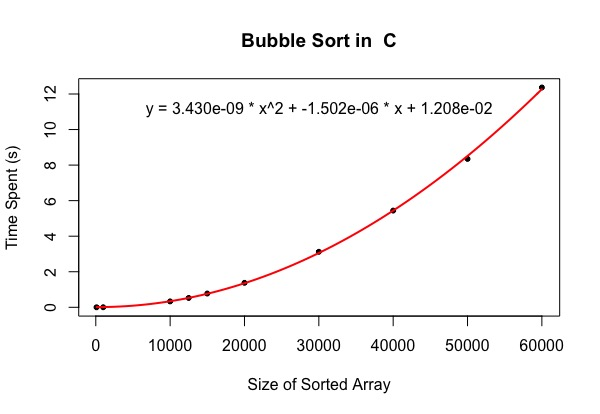
\includegraphics[width=0.6\textwidth]{resources/visualizations/bubblesortc.jpeg}
						\caption{Bubble Sort in C}
					\end{figure}
					
		 		\subsubsection{Merge Sort}
					\begin{figure}[H]
						\centering
						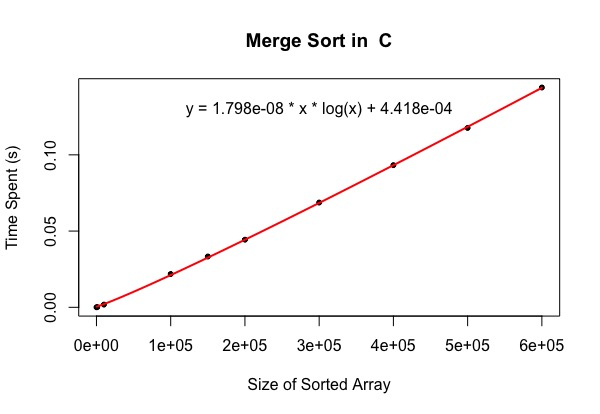
\includegraphics[width=0.6\textwidth]{resources/visualizations/mergesortc.jpeg}
						\caption{Merge Sort in C}
					\end{figure}
					
		 	\subsection{Python}
		 	
		 		\subsubsection{Bubble Sort}
					\begin{figure}[H]
						\centering
						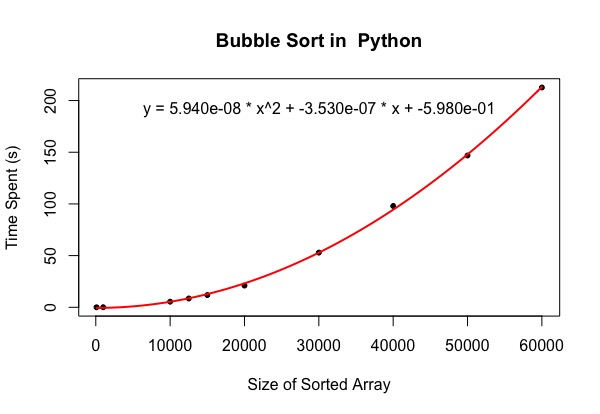
\includegraphics[width=0.6\textwidth]{resources/visualizations/bubblesortpython.jpeg}
						\caption{Bubble Sort in Python}
					\end{figure}
					
		 		\subsubsection{Merge Sort}
					\begin{figure}[H]
						\centering
						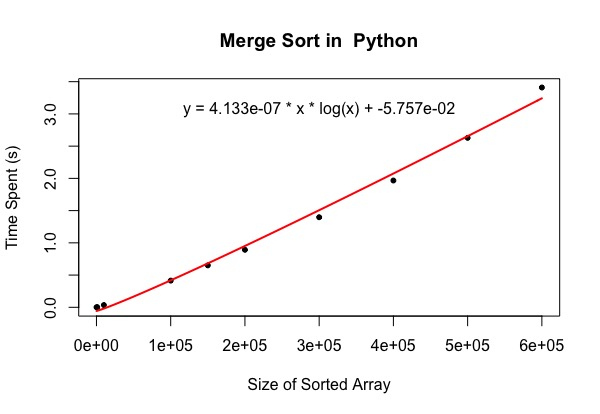
\includegraphics[width=0.6\textwidth]{resources/visualizations/mergesortpython.jpeg}
						\caption{Merge Sort in Python}
					\end{figure}
					
		    \subsection{Racket}
		    
		 		\subsubsection{Bubble Sort}
					\begin{figure}[H]
						\centering
						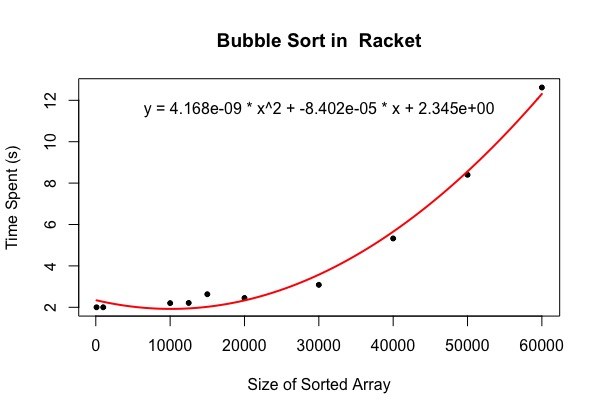
\includegraphics[width=0.6\textwidth]{resources/visualizations/bubblesortracket.jpeg}
						\caption{Bubble Sort in Racket}
					\end{figure}

		 		\subsubsection{Merge Sort}
					\begin{figure}[H]
						\centering
						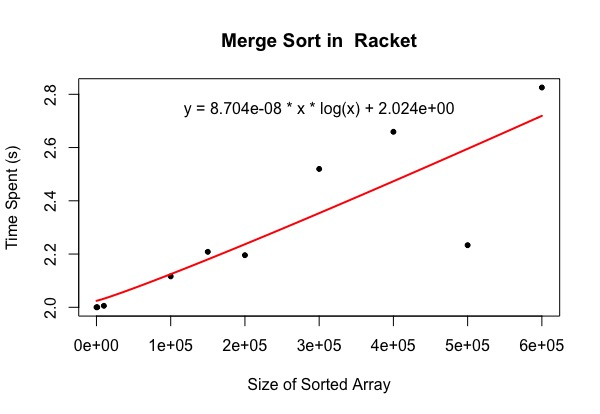
\includegraphics[width=0.6\textwidth]{resources/visualizations/mergesortracket.jpeg}
						\caption{Merge Sort in Racket}
					\end{figure}
					

	    \chapter{Mathematical Modeling}
	    Having visualized and predicted the model for all six datasets using R intelligence tools, let's use the tools we have learned in the Mathematical Modeling class to find an adequate model for all six datasets. First, we must point out that it is a well known fact that a bubble sort has a time complexity of $\mathcal{O}(n^2)$. This is because the inner loop of a bubble sort does $\mathcal{O}(n)$ work on each iteration, and the outer loop runs for $\mathcal{O}(n)$ iterations, so the total work is $\mathcal{O}(n^2)$. Second, the time complexity of a merge sort is $\mathcal{O}(n*log(n))$ as the merge sort always divides an array into two halves and takes linear time to merge two halves.
	    
			\section{C Language}
		 		\subsection{Bubble Sort}
		 		We know that the model for the time complexity of a bubble sorting algorithm is $\mathcal{O}(n^2)$. This means that a possible equation for this model is a polynomial of the second degree, i.e.
		 		\begin{ceqn}
					\begin{align}
		 				y = ax^2 + bx +c
					\end{align}
				\end{ceqn}
		 		To find the values of $a$, $b$ and $c$, we will be using the transformed Least-Squares fit method. Examples of the least-squares criterion appear easy to apply. However, it may be difficult for other types of functions. Let's apply the least-squares criterion to the model. Applying the least-squares criterion requires that we minimize:
		 		\begin{ceqn}
					\begin{align}
		 				S = \sum_{i=1}^{m}|y_i - f(x_i)|^2 = \sum_{i=1}^{m}|y_i - (ax_i^2+bx_i+c)|^2 \\
		 				= \sum_{i=1}^{m}|y_i - ax_i^2 - bx_i - c|^2
					\end{align}
				\end{ceqn}
				A necessary condition to optimize is setting the partial derivatives $\frac{\delta S}{\delta a}$, $\frac{\delta S}{\delta b}$ and $\frac{\delta S}{\delta c}$ to zero:
				\begin{equation}
					\begin{align}
		 				\frac{\delta S}{\delta a} = -2 \ \sum_{i=1}^{m}(y_i - ax_i^2-bx_i-c) \ \sum_{i=1}^{m}x_i^2 = 0\\
					\end{align}
				\end{equation}
				\begin{equation}
					\begin{align}
		 				\frac{\delta S}{\delta b} = -2 \ \sum_{i=1}^{m}(y_i - ax_i^2-bx_i-c) \ \sum_{i=1}^{m}x_i = 0\\
					\end{align}
				\end{equation}
				\begin{equation}
					\begin{align}
		 				\frac{\delta S}{\delta c} = -2 \ \sum_{i=1}^{m}(y_i - ax_i^2-bx_i-c) = 0\\
					\end{align}
				\end{equation}
				
				Once we solve the equations above, we get the three following equalities:
				\begin{equation}
					\begin{align}
		 				\sum_{i=1}^{m}ax_i^4 + \sum_{i=1}^{m}bx_i^3 + \sum_{i=1}^{m}cx_i^2 = \sum_{i=1}^{m}x_i^2y_i \\
					\end{align}
				\end{equation}
				\begin{equation}
					\begin{align}
		 				\sum_{i=1}^{m}ax_i^3 + \sum_{i=1}^{m}bx_i^2 + \sum_{i=1}^{m}cx_i = \sum_{i=1}^{m}x_iy_i\\
					\end{align}
				\end{equation}
				\begin{equation}
					\begin{align}
		 				 \sum_{i=1}^{m}ax_i^2 + \sum_{i=1}^{m}bx_i + c\ m = \sum_{i=1}^{m}y_i
					\end{align}
				\end{equation}
				
				We can conclude from the equalities above the following matrix:

				\begin{equation}
						\begin{bmatrix}
						\sum x_i^4 & \sum x_i^3 & \sum x_i^2 \\
						\sum x_i^3 & \sum x_i^2 & \sum x_i \\
						\sum x_i^2 & \sum x_i & m \\
						\end{bmatrix}
						\begin{bmatrix}
						a \\
						b \\
						c \\
						\end{bmatrix}
						=
						\begin{bmatrix}
						\sum x_i^2y_i \\
						\sum x_iy_i \\
						\sum y_i \\
						\end{bmatrix}
				\end{equation}
				
				Using computation tools (Excel and/or R), we find the values to fill the matrix, and the matrix becomes:
				\\
				\begin{equation}
						\begin{bmatrix}
						2.2825 \cdot 10^{+19} & 4.46329\cdot 10^{+14} & 9482260000 \\
						4.46329\cdot 10^{+14} & 9482260000 & 238600 \\
						9482260000 & 238600 & 10 \\
						\end{bmatrix}
						\begin{bmatrix}
						a \\
						b \\
						c \\
						\end{bmatrix}
						=
						\begin{bmatrix}
						77742172816 \\
						1519708.11 \\
						32.289977 \\
						\end{bmatrix} \\
				\end{equation}				
		 		
		 		Using Matlab, I found that the results of this system of equations is:
		 		
		 		\begin{equation}
		 			\begin{align}
						a = 3.430453052632288\cdot10^{-9}\\
						b = -1.507590425645456\cdot10^{-6}\\
						c = 0.012124031270596
		 			\end{align}
				\end{equation}
				
				We, therefore conclude that a quadratic model for the bubble sort in the C language is as follows:
				
				\begin{ceqn}
					\begin{align}
		 				y = 3.4304\cdot10^{-9}x^2 -1.5075\cdot10^{-6}x + 0.01212
					\end{align}
				\end{ceqn}
				
				We also notice that the model we found manually is almost equal to the one that R found, hence, we notice that R uses the least squares method in predicting models.
				
		 		\subsection{Merge Sort}
		 		
		 		We know that the model for the time complexity of a bubble sorting algorithm is $\mathcal{O}(n log(n))$. This means that a possible equation for this model is as follows, i.e.
		 		\begin{ceqn}
					\begin{align}
		 				y = a \cdot x log(x) + b
					\end{align}
				\end{ceqn}
		 		To find the values of $a$, and $b$, we will be using the transformed Least-Squares fit method. The least-squares criterion's application seemed easy to apply. Let's apply the least-squares criterion to the model. Applying the least-squares criterion requires that we minimize:
		 		\begin{ceqn}
					\begin{align}
		 				S = \sum_{i=1}^{m}|y_i - f(x_i)|^2 = \sum_{i=1}^{m}|y_i - (a \cdot x log(x) + b)|^2 \\
		 				= \sum_{i=1}^{m}|y_i - a \cdot x log(x) - b|^2
					\end{align}
				\end{ceqn}
				A necessary condition to optimize is setting the partial derivatives $\frac{\delta S}{\delta a}$ and $\frac{\delta S}{\delta b}$ to zero:
				\begin{equation}
					\begin{align}
		 				\frac{\delta S}{\delta a} = -2 \ \sum_{i=1}^{m}(y_i - a \cdot x log(x) - b) \ \sum_{i=1}^{m}x log(x) = 0\\
					\end{align}
				\end{equation}
				\begin{equation}
					\begin{align}
		 				\frac{\delta S}{\delta b} = 2 \ \sum_{i=1}^{m}(y_i - a \cdot x log(x) - b) = 0\\
					\end{align}
				\end{equation}
				
				Once we solve the equations above, we get the three following equalities:
				\begin{equation}
					\begin{align}
		 				 a\sum_{i=1}^{m}(x log(x))^2 + b\sum_{i=1}^{m}x log(x) = \sum_{i=1}^{m}x log(x)y_i\\
					\end{align}
				\end{equation}
				\begin{equation}
					\begin{align}
		 				 a\sum_{i=1}^{m}x log(x) + bm = \sum_{i=1}^{m}y_i\\
					\end{align}
				\end{equation}

				
				We can conclude from the equalities above the following matrix:

				\begin{equation}
						\begin{bmatrix}
						\sum (x log(x))^2 & \sum x log(x) \\
						\sum x log(x) & m \\
						\end{bmatrix}
						\begin{bmatrix}
						a \\
						b \\
						\end{bmatrix}
						=
						\begin{bmatrix}
						\sum x log(x) y_i\\
						\sum y_i \\
						\end{bmatrix}
				\end{equation}
				
				Using computation tools (Excel and/or R), we find the values to fill the matrix, and the matrix becomes:
				\\
				\begin{equation}
						\begin{bmatrix}
						2.98385 \cdot 10^{+13} & 12580155.81 \\
						12580155.81 & 10 \\
						\end{bmatrix}
						\begin{bmatrix}
						a \\
						b \\
						\end{bmatrix}
						=
						\begin{bmatrix}
						1240742.182 \\
						0.525181 \\
						\end{bmatrix} \\
				\end{equation}				
		 		
		 		Using Matlab, I found that the results of this system of equations is:
		 		
		 		\begin{equation}
		 			\begin{align}
						a = 4.139572714805141\cdot10^{-8}\\
						b = 4.416302609266260\cdot10^{-4}
		 			\end{align}
				\end{equation}
				
				We also notice that the model we found manually is almost equal to the one that R found, hence, we notice that R uses the least squares method in predicting models. model for the merge sort in the C language is as follows:
				
				\begin{ceqn}
					\begin{align}
		 				y = 4.1395\cdot10^{-8}xlog(x) + 4.4163\cdot10^{-4}
					\end{align}
				\end{ceqn}
				And, in case we want to replicate the R result, we would just need to substitute $log(x)$ = $\frac{ln(x)}{ln(10)}$ making the model also equal to:
				\begin{ceqn}
					\begin{align}
		 				y = 1.7977\cdot10^{-8}xln(x) + 4.4163\cdot10^{-4}
					\end{align}
				\end{ceqn}
				
				We also notice that the model we found manually is almost equal to the one that R found, hence, we notice that R uses the least squares method in predicting models.
		 		

		 	\section{Python}
		 		\subsection{Bubble Sort}
		 		Using our results from our analysis of the bubble sort in the C language, what we will reuse is the matrix equality to find a quadratic model for the bubble sort in Python:
		 		
				\begin{equation}
						\begin{bmatrix}
						\sum x_i^4 & \sum x_i^3 & \sum x_i^2 \\
						\sum x_i^3 & \sum x_i^2 & \sum x_i \\
						\sum x_i^2 & \sum x_i & m \\
						\end{bmatrix}
						\begin{bmatrix}
						a \\
						b \\
						c \\
						\end{bmatrix}
						=
						\begin{bmatrix}
						\sum x_i^2y_i \\
						\sum x_iy_i \\
						\sum y_i \\
						\end{bmatrix}
				\end{equation}
				
				Using computation tools (Excel and/or R), we find the values to fill the matrix, and the matrix becomes:
				\\
				\begin{equation}
						\begin{bmatrix}
						2.2825 \cdot 10^{+19} & 4.46329\cdot 10^{+14} & 9482260000 \\
						4.46329\cdot 10^{+14} & 9482260000 & 238600 \\
						9482260000 & 238600 & 10 \\
						\end{bmatrix}
						\begin{bmatrix}
						a \\
						b \\
						c \\
						\end{bmatrix}
						=
						\begin{bmatrix}
						1.34989\cdot 10^{+12} \\
						26364213.57 \\
						557.145961 \\
						\end{bmatrix} \\
				\end{equation}				
		 		
		 		Using Matlab, I found that the results of this system of equations is:
		 		
		 		\begin{equation}
		 			\begin{align}
						a = 5.939604847778412\cdot10^{-8}\\
						b = -3.448209508458306\cdot10^{-7}\\
						c = -0.598053936008141
		 			\end{align}
				\end{equation}
				
				We, therefore conclude that a quadratic model for the bubble sort in the Python language, is as follows:
				
				\begin{ceqn}
					\begin{align}
		 				y = 5.9396\cdot10^{-8}x^2 -3.4482\cdot10^{-7}x -0.5980
					\end{align}
				\end{ceqn}
				
				We also notice that the model we found manually is almost equal to the one that R found, hence, we notice that R uses the least squares method in predicting models.
				
		 		\subsection{Merge Sort}
		 		Using our results from our analysis of the merge sort in the C language, what we will reuse is the matrix equality to find a quadratic model for the merge sort in Python:
		 		
		 		\begin{equation}
						\begin{bmatrix}
						\sum (x log(x))^2 & \sum x log(x) \\
						\sum x log(x) & m \\
						\end{bmatrix}
						\begin{bmatrix}
						a \\
						b \\
						\end{bmatrix}
						=
						\begin{bmatrix}
						\sum x log(x) y_i\\
						\sum y_i \\
						\end{bmatrix}
				\end{equation}
				
				Using computation tools (Excel and/or R), we find the values to fill the matrix, and the matrix becomes:
				\\
				\begin{equation}
						\begin{bmatrix}
						2.98385 \cdot 10^{+13} & 12580155.81 \\
						12580155.81 & 10 \\
						\end{bmatrix}
						\begin{bmatrix}
						a \\
						b \\
						\end{bmatrix}
						=
						\begin{bmatrix}
						27673914.82 \\
						11.397183 \\
						\end{bmatrix} \\
				\end{equation}				
		 		
		 		Using Matlab, I found that the results of this system of equations is:
		 		
		 		\begin{equation}
		 			\begin{align}
						a = 9.517296343438738\cdot10^{-7}\\
						b = -0.057572408904026
		 			\end{align}
				\end{equation}
				
				We also notice that the model we found manually is almost equal to the one that R found, hence, we notice that R uses the least squares method in predicting models. model for the merge sort in the Python language is as follows:
				
				\begin{ceqn}
					\begin{align}
		 				y = 9.5172\cdot10^{-7}xlog(x) -0.05757
					\end{align}
				\end{ceqn}
				And, in case we want to replicate the R result, we would just need to substitute $log(x)$ = $\frac{ln(x)}{ln(10)}$ making the model also equal to:
				\begin{ceqn}
					\begin{align}
		 				y = 4.1333\cdot10^{-7}xln(x) -0.05757
					\end{align}
				\end{ceqn}
				
				We also notice that the model we found manually is almost equal to the one that R found, hence, we notice that R uses the least squares method in predicting models.
		 		
		 		
		 		
		 		
		    \section{Racket}
		 		\subsection{Bubble Sort}
		 		Using our results from our analysis of the bubble sort in the C language, what we will reuse is the matrix equality to find a quadratic model for the bubble sort in Racket:
		 		
				\begin{equation}
						\begin{bmatrix}
						\sum x_i^4 & \sum x_i^3 & \sum x_i^2 \\
						\sum x_i^3 & \sum x_i^2 & \sum x_i \\
						\sum x_i^2 & \sum x_i & m \\
						\end{bmatrix}
						\begin{bmatrix}
						a \\
						b \\
						c \\
						\end{bmatrix}
						=
						\begin{bmatrix}
						\sum x_i^2y_i \\
						\sum x_iy_i \\
						\sum y_i \\
						\end{bmatrix}
				\end{equation}
				
				Using computation tools (Excel and/or R), we find the values to fill the matrix, and the matrix becomes:
				\\
				\begin{equation}
						\begin{bmatrix}
						2.2825 \cdot 10^{+19} & 4.46329\cdot 10^{+14} & 9482260000 \\
						4.46329\cdot 10^{+14} & 9482260000 & 238600 \\
						9482260000 & 238600 & 10 \\
						\end{bmatrix}
						\begin{bmatrix}
						a \\
						b \\
						c \\
						\end{bmatrix}
						=
						\begin{bmatrix}
						79869972206 \\
						1623117.854 \\
						42.925107 \\
						\end{bmatrix} \\
				\end{equation}				
		 		
		 		Using Matlab, I found that the results of this system of equations is:
		 		
		 		\begin{equation}
		 			\begin{align}
						a = 4.168065707722193\cdot10^{-9}\\
						b = -8.402491569874184\cdot10^{-5}\\
						c = 2.345076914801395
		 			\end{align}
				\end{equation}
				
				We, therefore conclude that a quadratic model for the bubble sort in the Racket language, is as follows:
				
				\begin{ceqn}
					\begin{align}
		 				y = 4.1680\cdot10^{-9}x^2 -8.4024\cdot10^{-5}x +2.3450
					\end{align}
				\end{ceqn}
				
				We also notice that the model we found manually is almost equal to the one that R found, hence, we notice that R uses the least squares method in predicting models.
		 		\subsection{Merge Sort}
		 		
		 		Using our results from our analysis of the merge sort in the C language, what we will reuse is the matrix equality to find a quadratic model for the merge sort in Racket:
		 		
		 		\begin{equation}
						\begin{bmatrix}
						\sum (x log(x))^2 & \sum x log(x) \\
						\sum x log(x) & m \\
						\end{bmatrix}
						\begin{bmatrix}
						a \\
						b \\
						\end{bmatrix}
						=
						\begin{bmatrix}
						\sum x log(x) y_i\\
						\sum y_i \\
						\end{bmatrix}
				\end{equation}
				
				Using computation tools (Excel and/or R), we find the values to fill the matrix, and the matrix becomes:
				\\
				\begin{equation}
						\begin{bmatrix}
						2.98385 \cdot 10^{+13} & 12580155.81 \\
						12580155.81 & 10 \\
						\end{bmatrix}
						\begin{bmatrix}
						a \\
						b \\
						\end{bmatrix}
						=
						\begin{bmatrix}
						31445483.03 \\
						22.763856 \\
						\end{bmatrix} \\
				\end{equation}				
		 		
		 		Using Matlab, I found that the results of this system of equations is:
		 		
		 		\begin{equation}
		 			\begin{align}
						a = 2.004070590880563\cdot10^{-7}\\
						b = 2.024270397124837
		 			\end{align}
				\end{equation}
				
				We also notice that the model we found manually is almost equal to the one that R found, hence, we notice that R uses the least squares method in predicting models. model for the merge sort in the Racket language is as follows:
				
				\begin{ceqn}
					\begin{align}
		 				y = 2.0040705\cdot10^{-7}xlog(x) + 2.02427
					\end{align}
				\end{ceqn}
				And, in case we want to replicate the R result, we would just need to substitute $log(x)$ = $\frac{ln(x)}{ln(10)}$ making the model also equal to:
				\begin{ceqn}
					\begin{align}
		 				y = 8.7035\cdot10^{-8}xln(x) + 2.02427
					\end{align}
				\end{ceqn}
				
				We also notice that the model we found manually is almost equal to the one that R found, hence, we notice that R uses the least squares method in predicting models.
		 		
		 		


		\chapter{Conclusion}
		
		\section{Recapitulation}
		In this research paper, I have reported in detail all phases of my research, starting from the data collection itself, to plotting the data, to modeling it both manually and digitally, and the model results seems conclusive and correct. Now, in order to see how models compare to each other, here are two graphs with all models that will help us grasp graphically how each language compares to the other two languages for both sorting algorithms separately and unitedly.
		
			\begin{figure}[H]
				\centering
				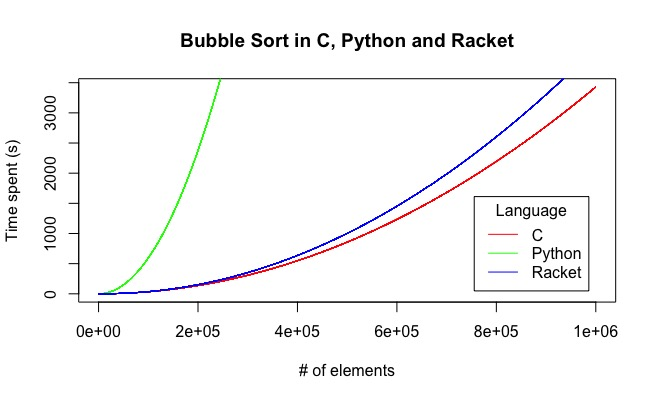
\includegraphics[width=0.8\textwidth]{resources/visualizations/bubblesortinalllangs.jpeg}
						\caption{Comparison of Bubble Sort in different languages}
			\end{figure}
			
			\begin{figure}[H]
				\centering
				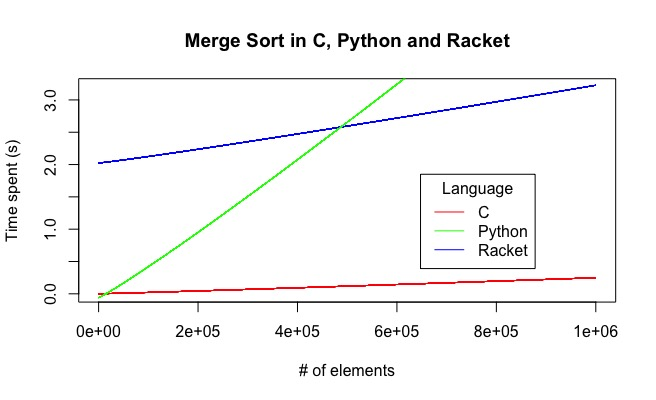
\includegraphics[width=0.8\textwidth]{resources/visualizations/mergesortinalllangs.jpeg}
						\caption{Comparison of Merge Sort in different languages}
			\end{figure}
			
		And finally, just to ensure graphically that a merge sorting algorithm is much much faster than a bubble sorting approach, here's a graph of all bubble sorts vs. all merge sorts.
		
			\begin{figure}[H]
				\centering
				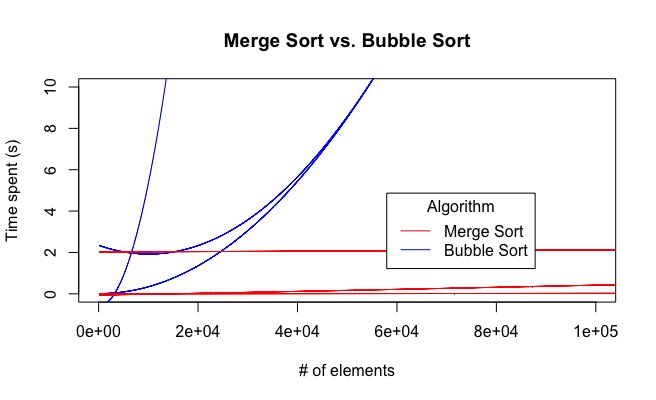
\includegraphics[width=0.8\textwidth]{resources/visualizations/bubblevsmergealllangs.jpeg}
						\caption{Comparison of Merge Sort and Bubble Sort}
			\end{figure}
		
	    \section{Speed Differences and Reasons}
	    We can conclude from both the graphs and the numerical data that the fastest language by far in terms of sorting regardless of which algorithm is C. That is what I expected as C is a very low-level programming language that has a very low-level array definition that makes array mutable (in terms of their contents). \\
	    This makes moving data around in one array very easy through indexing and looping. The next fastest language is up to debate as both other languages, Python and Racket, are mostly interpreted (especially in our experimentation) which makes them inherently slower than compiled languages like C.\\
	    Additionally, the models and the experimental results show inconclusive data when it comes to second best, as Racket is faster than Python in terms of merge sorting, while it is slower than Python in bubble sorting.\\
	    The explanation I found for there being better performance in Racket than in Python is that merge sorting is subcomposed of many list constructions, which is what Racket and other LISP (List Processing) languages are designed to do best.
	    This explanation also works for showing why a bubble sort is slower in Racket than it is in Python. And that is because Racket is functional. It was designed to deal with function, and process lists, making there no simple and fast way to access an element at a specific index.
	    As a conclusion, it seems that all results and these time complexity based models are valid and adequate for predicting how these languages would run sorting algorithms in terms of the size of the sample.\\
	    
	    	 			    
	\newpage

		\bibliographystyle{plain} 	
		\bibliography{resources/references}

\end{document} % This is the end of the document